\title{Bluetooth Mesh Platform für IoT Anwendungen}
\team{%
	Cyrill Horath,
	Raffael Anklin,
    Robin Bobst}

\projtype{Pro5E}

\coaches{%
    Matthias Meier ,
    Manuel Di Cerbo}

\fssummary{
    Irgend eine Einleitung die alle umhaut.}

\fsgraphics{
    \begin{minipage}{0.5\textwidth}
        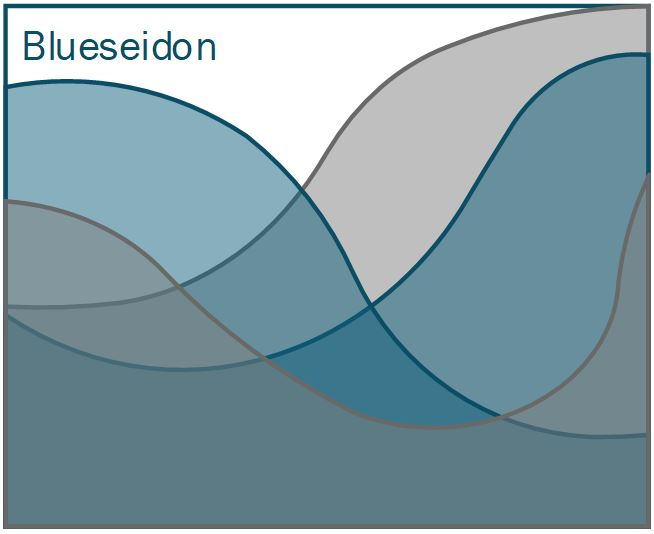
\includegraphics[height=60mm]{images/Blueseidon_Titelbild}
       % \graphicscaption{Ender 3 Pro}
    \end{minipage}%
    \begin{minipage}{0.5\textwidth}
        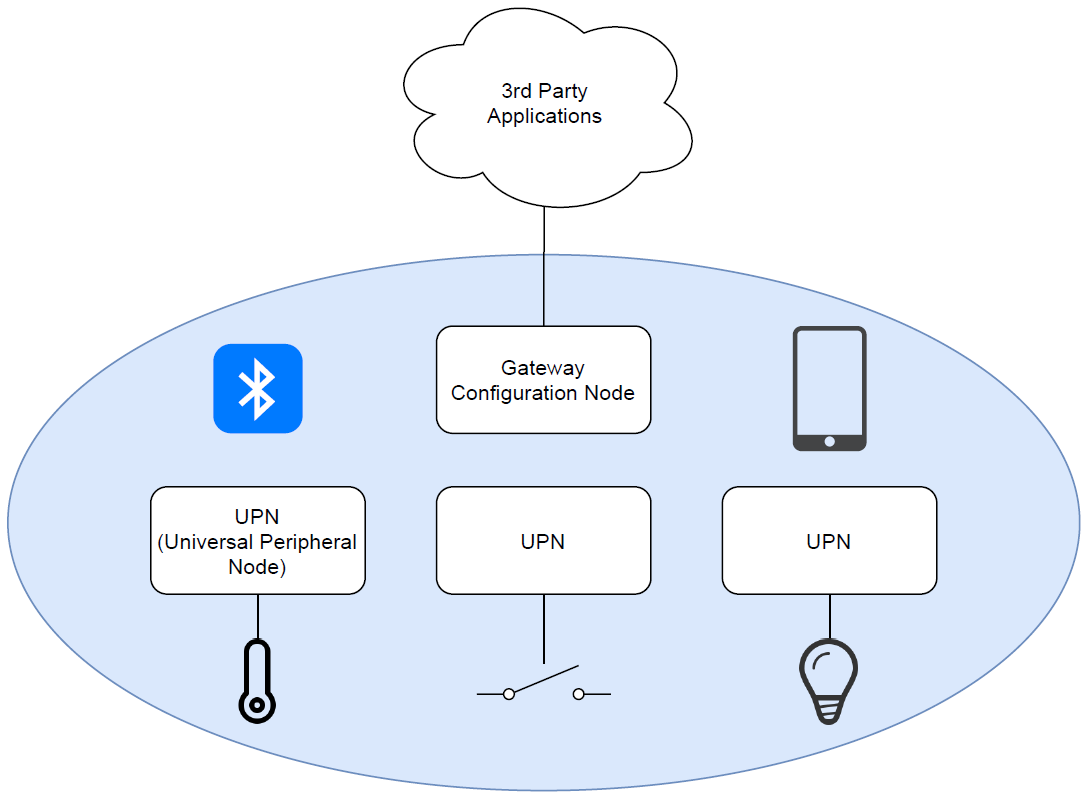
\includegraphics[height=60mm]{images/Grobkonzept_Schema.PNG}
        %\graphicscaption{Steuerungsprint}
    \end{minipage}
}

\fscontent{
    \section{Wireless}
    In der heutigen Entwicklung ist der Bedarf an drahtlosen Sensoren und Aktoren gestiegen. In vielen Bereichen werden kleine unabhängige Systeme benötigt. Sei es in der Heimautomation (Lichtschalter, Temperaturfühler, etc.), der Industrie (Produktionserfassung, Lagerbewirtschaftung, etc.) oder der Landwirtschaft (Feuchtigkeitsmessung, Bewässerungssysteme, etc.). Es existieren diverse Lösungsansätze solche Wireless Sensor Networks (WSN) zu realisieren. Eine Möglichkeit ist das Vernetzen der Geräte über das weit verbreitet Bluetooth Protokoll. Dazu wurde im Jahr 2017 der Bluetooth Mesh Standard vorgestellt in welchem Knoten ein MeshNetzwerk bilden. Mesh-Netzwerke haben die Eigenschaft die Abdeckung mit jedem zusätzlichen Knoten zu erweitern indem sie die Daten jeweils vom einen zum anderen Knoten weiterleiten.

    \section{Blueseidon}
  	Ziel dieses Projektes ist es, eine \textit{Bluetooth Mesh Plattform} zu entwickeln, die es ermöglicht ein Netzwerk vereinfacht aufzubauen und zu konfigurieren. Die Plattform soll dem Endanwender die Möglichkeit bieten eine beliebige Anzahl Knoten einzubinden und diese je nach Anwendung zu konfigurieren. Ein weiteres Ziel dieses Projektes ist es die Bluetooth Mesh Knoten möglichst netzunabhängig zu betreiben. Dazu soll sogenanntes Energy Harvesting eingesetzt werden. Energy Harvesting steht als Überbegriff für die Energiegewinnung aus der Umgebung, wozu beispielsweise Solarenergie, Vibrationsenergie, Thermische Energie aber auch die Energie von Elektromagnetischen Wellen zählt. 

    \section{Node-Red (Bedienung?)}
	Evtl Node-Red beschreiben? \\
   \\
   \begin{minipage}{0.6\textwidth}
   	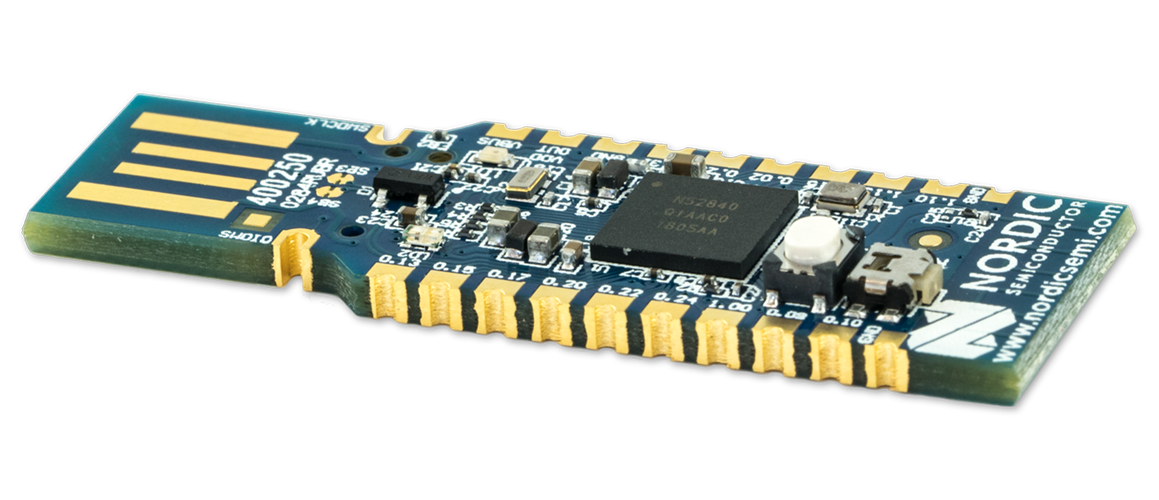
\includegraphics[height=25mm]{images/nRF52840_Dongle.png}
   \end{minipage}
}

\infobox{Highlights}{%
    \footnotesize
    \setlength\tabcolsep{2pt}
   	\begin{itemize}
   	\item nRF52840
   	\item ...
	\end{itemize}
}
